\documentclass[11pt,a4paper]{article}
\usepackage[margin=2.3cm]{geometry}
\usepackage[T1]{fontenc}
\usepackage{lmodern,microtype,amsmath,amssymb,booktabs,graphicx,caption,hyperref,xcolor,float}
\usepackage[section]{placeins}
\definecolor{navy}{HTML}{173B61}
\hypersetup{colorlinks=true,linkcolor=navy,citecolor=navy,urlcolor=navy,pdftitle={Spatial Temperature Interpolation in Gilan Province},pdfauthor={Seyedamir Rahmani}}
\graphicspath{{../figures/}{figures/}}
\setlength{\parindent}{0pt}
\setlength{\parskip}{5pt}
\captionsetup{font=small,labelfont=bf}
\newcommand{\degC}{\ensuremath{{}^{\circ}\mathrm{C}}}
\title{\textbf{A Comparative Study of Spatial Interpolation Methods for Replicating Temperature Patterns in Gilan Province, Iran}}
\author{Seyedamir Rahmani\\\small Faculty of Computer Science and Mathematics\\\small Iran University of Science and Technology (IUST)\\[3pt]\small Supervisor: Mahboubeh Molavi-Arabshahi}
\date{Undergraduate research, Spring 2025\\ Revised November 2026}
\begin{document}
\maketitle
\begin{abstract}
This supervised undergraduate study adapts the comparative evaluation of Yang and Xing (2021) to annual and seasonal ERA5 temperature reconstruction in Gilan Province. Monthly data for 2015--2024 yield 23 masked spatial sampling locations. Five fixed configurations are evaluated: elevation-adjusted inverse distance weighting (IDW), two radial basis function (RBF) kernels, spherical ordinary kriging and EBK-inspired local kriging. All 575 leave-one-location-out predictions completed without failure. Multiquadric RBF achieves an annual mean absolute error (MAE) of 0.323~\degC, root mean squared error (RMSE) of 0.425~\degC, and Nash--Sutcliffe efficiency (NSE) of 0.971. Winter IDW and multiquadric RBF MAEs are nearly equal. Entropy-weighted TOPSIS rankings are sensitive to criterion selection, including a winter winner reversal. The results characterize reconstruction of withheld reanalysis values rather than independent weather-station validation and do not establish general algorithm superiority.
\end{abstract}
\smallskip\textbf{Keywords:} spatial interpolation; ERA5; radial basis functions; kriging; cross-validation; TOPSIS

\section{Introduction}
Spatial temperature reconstruction provides a numerical-analysis setting for comparing distance weighting, radial kernel expansions and covariance-based prediction. This study compares fixed interpolation configurations under a common withholding protocol in Gilan Province, using ERA5 spatial data and a provincial mask. The evaluation framework and entropy-weighted TOPSIS are adapted from Yang and Xing~\cite{yang}, whose original application concerned rainfall in Chongqing. The objective is comparative evaluation, not the development of a novel interpolation algorithm.

\section{Related work}
Yang and Xing~\cite{yang} compared six interpolation methods using leave-one-out cross-validation (LOOCV), error measures, Spearman correlation and entropy-weighted TOPSIS. Their CRS RBF, barrier methods, station observations and commercial GIS methods are not replicated here. This adaptation changes the variable, study area, data source, temporal definitions and numerical implementations. SciPy documents the raw kernel expansion used here~\cite{rbf}; established empirical Bayesian kriging (EBK) uses repeated semivariogram simulation and weighting~\cite{ebk}, distinct from the local pseudo-target sampler in this study. No transfer of the original method hierarchy to temperature reconstruction is assumed.

\section{Study area and data}
The ERA5 NetCDF input contains 120 monthly timestamps from January 2015 to December 2024 on a $9\times9$ subset of the $0.25^\circ$ grid. Strict interior containment with GADM 4.1~\cite{gadm} retains 23 distinct grid locations, or 2,760 location-month records, with no missing temperatures or geopotential values. ERA5 is a reanalysis product~\cite{era5}, not independent station measurements. Temperatures are converted by $T_C=T_K-273.15$; geopotential height is $h=z/9.80665$ in metres.

Annual climatology equally weights all 120 monthly means; seasonal means use MAM, JJA, SON and pooled DJF (30 means each). Monthly values are not weighted by days per month. DJF pools calendar-range months rather than estimating complete cross-year winters. No missing data are imputed. Coordinates are projected from longitude and latitude to WGS84/UTM zone 39N, in kilometres. The $0.005^\circ$ geographic target grid controls visual sampling, not the information content of the original grid.

External elevation data are needed only for IDW mapping. The replacement uses the SRTM GL1 version~3 product at 1 arc-second spacing (approximately 30~m), in WGS84 horizontal coordinates and EGM96 orthometric metres. Six tiles (N36E049, N36E050, N37E048, N37E049, N37E050 and N38E048) were acquired on 27 November 2026 through OpenTopography's public distribution~\cite{opentopo}; the USGS product overview is given in~\cite{srtm}. This is not an EarthExplorer acquisition, and byte-level identity to a separate USGS GeoTIFF download is not asserted. Each tile has $3601\times3601$ postings; metadata and SHA-256 hashes are recorded with the project. The preprocessing pipeline checks the native raster lattice, merges tiles, clips to a padded extent and bilinearly samples 57,536 target centres without filling NoData; these are point samples, not cell averages. The SRTM orthometric elevation and ERA5 geopotential height~\cite{ecmwf} are distinct height quantities; combining them in a fixed lapse-rate model is an approximation, not an exact vertical-datum conversion.

\textit{Revision note.} The original 2025 external DEM raster and acquisition metadata are unavailable. During the November 2026 reproducibility revision, it was replaced with documented SRTM GL1 elevations and the IDW maps were regenerated. This replacement was not used in the original 2025 study. The historical CSV is preserved privately for comparison; material numerical corrections are recorded in the project changelog.

\section{Methodology}
\subsection{Interpolation configurations}
\paragraph{Elevation-adjusted inverse distance weighting.} With training temperatures $T_i$, elevations $h_i$, distances $d_i$ and lapse rate $L=-0.0065$~\degC/m, the estimate is
\begin{equation}
\widehat T(x)=\frac{\sum_i d_i^{-2}(T_i-Lh_i)}{\sum_i d_i^{-2}}+Lh(x).
\end{equation}
Coincident locations receive exact spatial weight. The lapse rate is fixed, not estimated from withheld temperatures. LOOCV uses available ERA5 grid heights at withheld locations; full map generation uses external target elevations matched by coordinates. Only IDW uses elevation, so the comparison concerns configurations with differing covariate use.

\paragraph{Radial basis functions.} The expansion is $\widehat T(x)=\sum_i w_i\phi(\lVert x-x_i\rVert)$, with weights fitted on training coordinates and values. The two kernels are
\begin{align}
\phi_{\mathrm{TP}}(r)&=r^2\log r,\quad \phi_{\mathrm{TP}}(0)=0,\\
\phi_{\mathrm{MQ}}(r)&=\sqrt{1+(r/\epsilon)^2}.
\end{align}
The original SciPy \texttt{Rbf} implementation~\cite{rbf} uses zero smoothing and the training-coordinate default $\epsilon$. No affine polynomial tail is included, so the thin-plate kernel is not claimed to minimize the classical bending-energy functional. Identical configurations are used for mapping and validation, with fold-specific training sets; neither kernel is tuned and then presented as independently validated on the same scores.

\paragraph{Ordinary kriging.} The spherical covariance is
\begin{equation}
C(h)=\begin{cases}s(1-1.5h/a+0.5(h/a)^3),&h<a,\\0,&h\geq a,\end{cases}
\end{equation}
where $s$ is training variance, range $a=55.5$ km and nugget is zero. The range is a fixed latitude-based approximation to the original 0.5-degree scale, not a fitted optimum. The augmented system
\begin{equation}
\begin{bmatrix}C&\mathbf{1}\\\mathbf{1}^\top&0\end{bmatrix}\begin{bmatrix}w\\\lambda\end{bmatrix}=\begin{bmatrix}c\\1\end{bmatrix}
\end{equation}
is symmetric indefinite and solved accordingly, with checked least-squares fallback, no diagonal regularization, and verification of the unit-sum constraint.

\paragraph{EBK-inspired local kriging.} At most 15 nearest training locations are selected. Rank-normal temperatures use average ranks and $\Phi^{-1}(\mathrm{rank}/(n+1))$. An empirical semivariogram includes the maximum pair distance; the model has exponential covariance. Parameters $\theta=(\text{nugget},\text{partial sill},\text{scale})$ follow a bounded pseudo-target
\begin{equation}
\pi(\theta)\propto\exp\left[-\sum_j(\gamma_{\mathrm{emp},j}-\gamma_{\theta,j})^2\right].
\end{equation}
Nugget and partial-sill bounds are $[0,2]$ and $[0.01,4]$ in squared normal-score units; the scale bound is $[5,300]$ km. Additive Gaussian proposal standard deviations are 0.005 and 0.05 in the corresponding variance units, and 5 km for scale. Out-of-bound proposals are rejected; symmetry yields acceptance probability $\min(1,\exp(\log\pi(\theta')-\log\pi(\theta)))$. Each chain runs 150 iterations with 75 discarded. Thirty retained parameter vectors are resampled with replacement. A prediction for each selected model is inverse-transformed using the unique training score/value pairs and then averaged. Inverse tails clamp to the training range. Shared neighborhoods reuse deterministic chains; independent NumPy seed streams depend on fold and neighbor indices. Finite bounds define a proper pseudo-target, not a calibrated likelihood. Short chains do not establish convergence, and the estimator is not conventional EBK, an unbiased back-transform, or a predictive uncertainty model.

\subsection{Validation and evaluation}
Each of 23 locations is withheld once in each of five climatologies. All methods use the same training and withheld locations. Variance, normal scores, inverse transforms, empirical variograms and sampled parameters are fitted from training temperatures only. Geographic masks, elevations and the fixed lapse rate use no withheld temperatures. Nonfinite predictions invalidate affected aggregates instead of being silently dropped. The saved experiment contains 575 finite predictions and no failures.

For $e_i=\widehat T_i-T_i$, the primary measures are
\begin{align}
\mathrm{MAE}&=n^{-1}\sum_i|e_i|, &\mathrm{RMSE}&=\sqrt{n^{-1}\sum_i e_i^2},\\
\mathrm{NSE}&=1-\frac{\sum_i e_i^2}{\sum_i(T_i-\overline T)^2},
\end{align}
with NSE following Nash and Sutcliffe~\cite{nash}. Spearman correlation is computed from average ranks~\cite{spearman}; Pearson is diagnostic. Historical percentage errors are $100\,\mathrm{mean}(|e_i/T_i|)$ (MAPE) and $200\,\mathrm{mean}(|e_i|/(|T_i|+|\widehat T_i|))$ (SMAPE), only where denominators are nonzero. These are sensitive to the arbitrary zero of Celsius and are not primary metrics. Minimum absolute error is an individual statistic, not MAE. No inferential p-values are emphasized for the spatially dependent sample.

\subsection{Entropy-weighted TOPSIS}
For benefit-oriented min--max normalized scores $u_{ij}$, let $p_{ij}=u_{ij}/\sum_i u_{ij}$. Entropy and weight are
\begin{equation}
H_j=-\frac{\sum_i p_{ij}\log p_{ij}}{\log n},\qquad w_j=\frac{1-H_j}{\sum_k(1-H_k)}.
\end{equation}
Zero probabilities contribute zero entropy and constant criteria receive zero weight. Weighted column extrema define the positive and negative ideals. Closeness is $D_-/(D_++D_-)$, with wholly tied alternatives assigned 0.5. Min--max scaling supports negative NSE. Historical criteria are MSE, MAE, MAPE, SMAPE and NSE; primary criteria are MAE, RMSE and Spearman; reduced criteria are MAE and Spearman. NSE is affine in MSE within a period. Entropy weighting does not remove redundancy, motivating the reduced set.

\section{Results}
\subsection{Spatial reconstruction}
The figures show all five configurations, including elevation-adjusted IDW using the replacement SRTM data. These maps show reconstructed climatologies rather than measured temperatures; the fine grid does not imply fine-resolution validation. At the same 57,536 target centres, replacement minus historical elevation has a mean of $-2.02$~m, mean absolute difference of 6.43~m, RMSE of 8.81~m and maximum absolute difference of 84~m; elevation correlation is 0.99995. The corresponding IDW map changes have mean $+0.013$~\degC, mean absolute change 0.042~\degC, RMSE 0.057~\degC and maximum absolute change 0.546~\degC, identically across periods. These differences follow $\Delta\widehat T=L\Delta h$ for unchanged training inputs. Larger differences are localized rather than a uniform height offset. The unknown historical source and vertical datum prevent attribution to a specific processing step. The other four map configurations, all 575 held-out predictions, 25 aggregate metric records and 75 TOPSIS ranking records are unchanged.
\begin{figure}[htbp]
\centering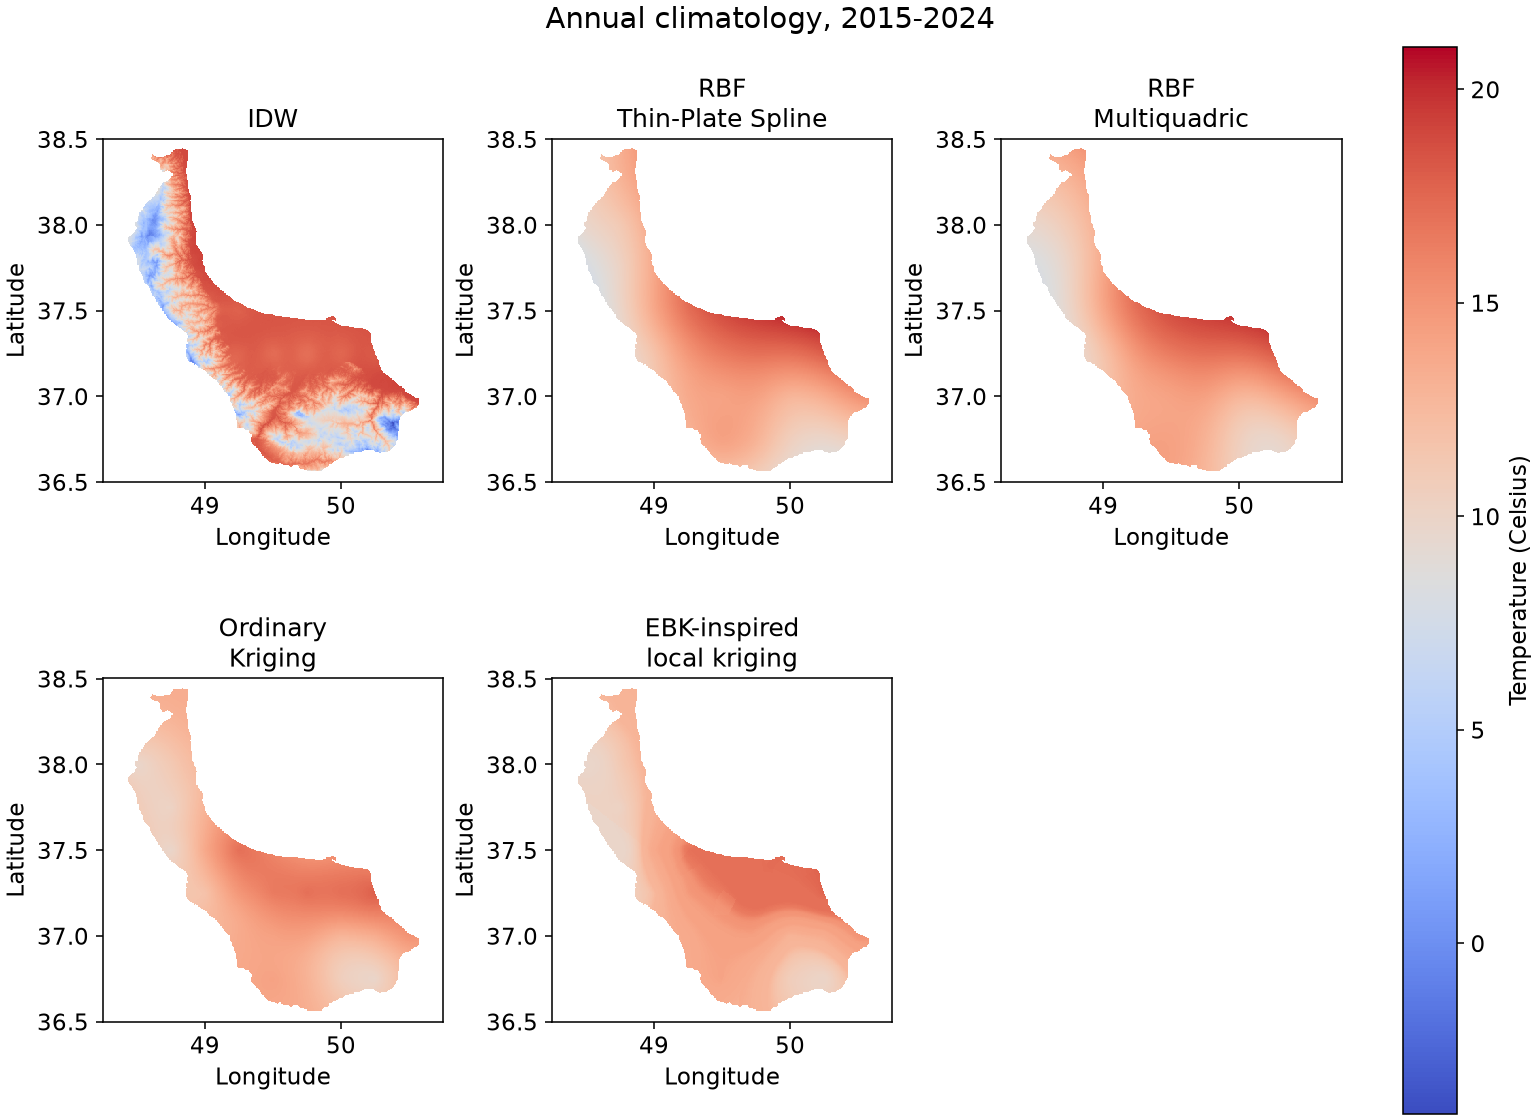
\includegraphics[width=\linewidth]{temperature_maps/annual.png}
\caption{Annual temperature reconstruction for 2015--2024 (five configurations; IDW uses replacement SRTM elevations; common colour scale in \degC).}\label{fig:annual}
\end{figure}
\subsection{Held-out prediction accuracy}
Table~\ref{tab:annual} gives the annual metrics, and Table~\ref{tab:season} summarizes seasonal MAE. Multiquadric RBF has the lowest MAE for annual, spring, summer and fall climatologies. Winter MAEs are almost identical for IDW (0.409452~\degC) and multiquadric RBF (0.409866~\degC); the latter has lower winter RMSE. The tested ordinary kriging configuration has larger errors, not evidence that the whole method class is unsuitable.
\begin{table}[htbp]\centering\caption{Annual LOOCV metrics (23 predictions per method; MAE and RMSE in \degC).}\label{tab:annual}\begin{tabular}{lrrrr}\toprule Method & MAE & RMSE & NSE & Spearman\\\midrule
IDW & 0.746 & 0.886 & 0.874 & 0.973\\
RBF thin-plate & 0.612 & 0.852 & 0.884 & 0.967\\
RBF multiquadric & 0.323 & 0.425 & 0.971 & 0.967\\
Ordinary kriging & 1.099 & 1.423 & 0.675 & 0.896\\
EBK-inspired local kriging & 1.002 & 1.290 & 0.733 & 0.864\\
\bottomrule\end{tabular}\end{table}
\begin{table}[htbp]\centering\caption{Mean absolute error by climatology (\degC).}\label{tab:season}\begin{tabular}{lrrrrr}\toprule Method & Annual & Spring & Summer & Fall & Winter\\\midrule
IDW & 0.7456 & 1.1677 & 0.9395 & 0.7291 & 0.4095\\
RBF thin-plate & 0.6124 & 0.5817 & 0.6335 & 0.6489 & 0.7200\\
RBF multiquadric & 0.3227 & 0.3743 & 0.3841 & 0.3946 & 0.4099\\
Ordinary kriging & 1.0993 & 0.8838 & 0.9881 & 1.1312 & 1.4474\\
EBK-inspired local kriging & 1.0022 & 0.7576 & 1.0112 & 1.2207 & 1.3701\\
\bottomrule\end{tabular}\end{table}
\begin{figure}[htbp]\centering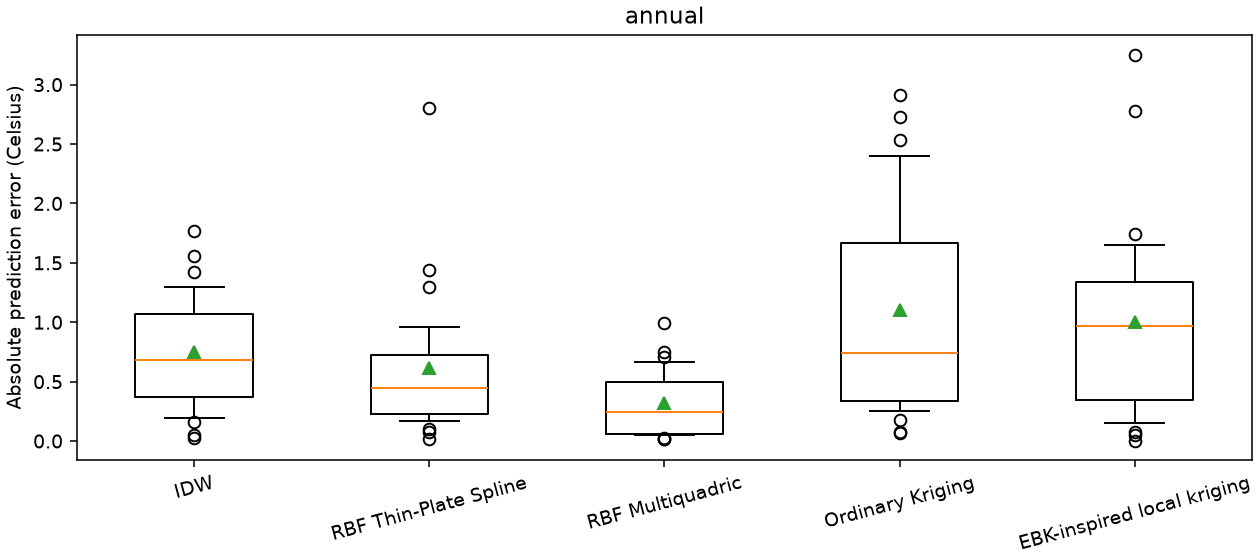
\includegraphics[width=\linewidth]{error_analysis/annual.png}\caption{Annual absolute prediction errors. Boxes show interquartile ranges, whiskers the 10th--90th percentiles and triangles the means.}\end{figure}
\begin{figure}[htbp]\centering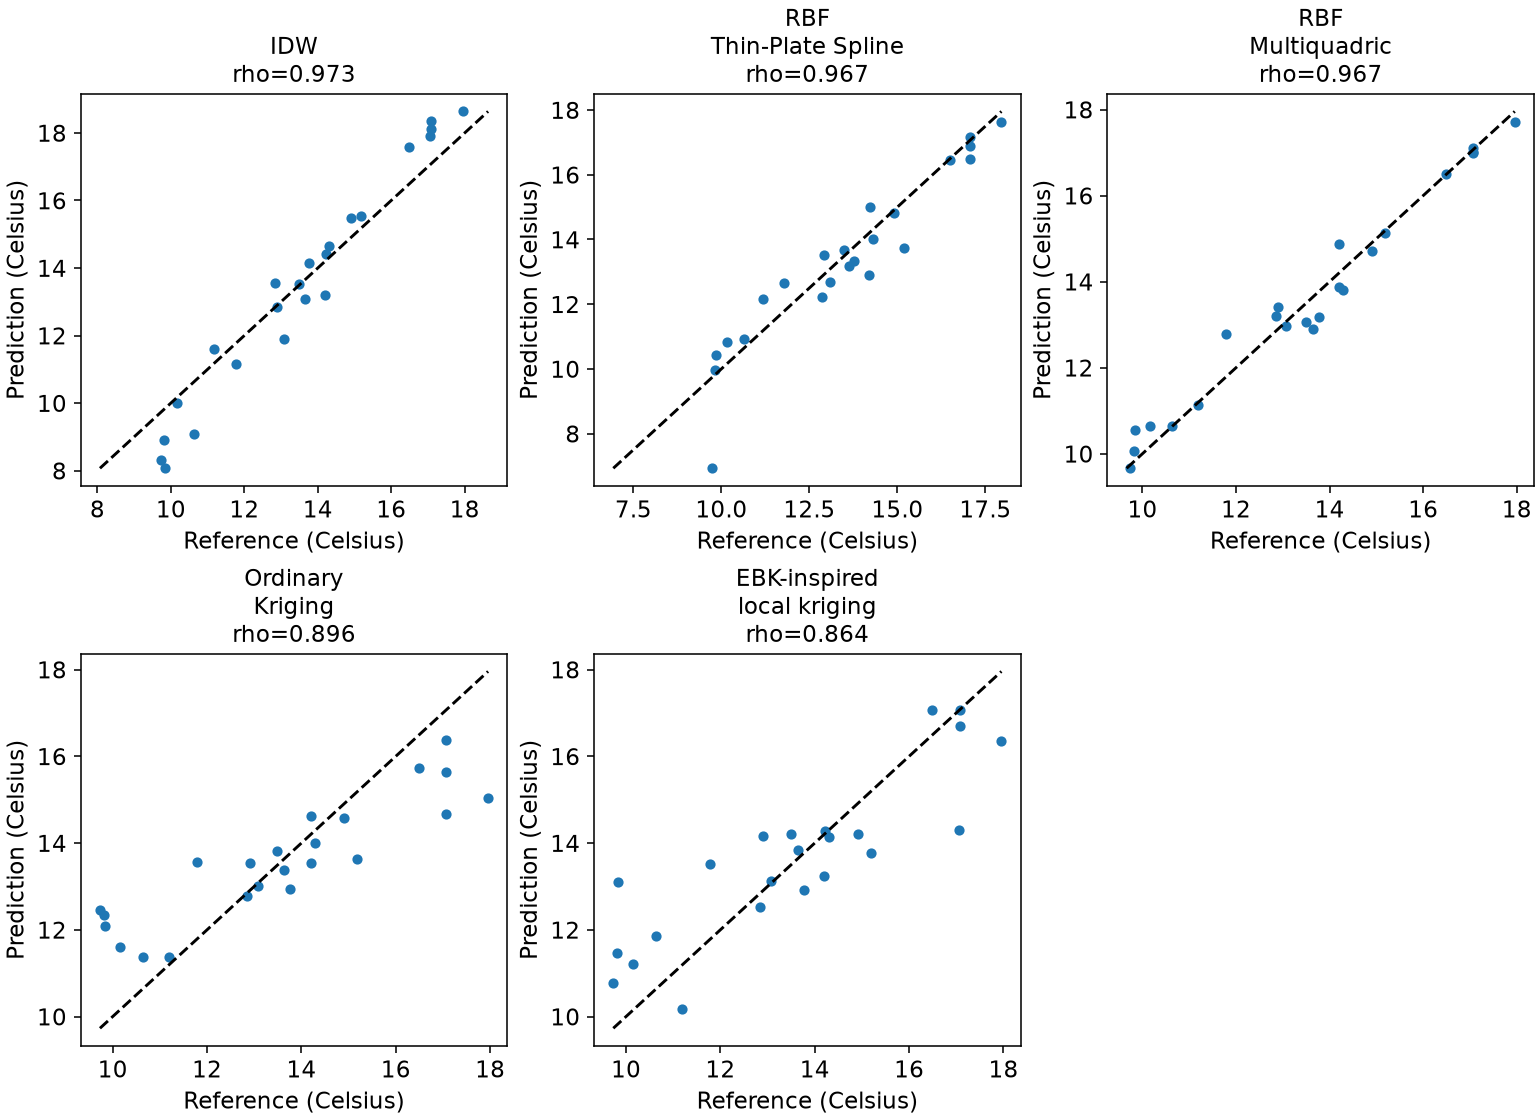
\includegraphics[width=\linewidth]{correlation/annual.png}\caption{Annual reference versus withheld predictions, with identity lines and descriptive Spearman correlations.}\end{figure}
\subsection{Ranking sensitivity} Multiquadric RBF ranks first in every period under primary and reduced criteria. The historical criteria instead rank IDW first in winter, driven in part by Celsius percentage errors. Annual ordinary and EBK-inspired kriging swap fourth/fifth positions between historical and primary sets; lower spring ranks also change. The closeness scores are internal decision scores, not probabilities of superiority.
\begin{table}[htbp]\centering\caption{TOPSIS rank sensitivity. Each cell gives historical / primary / reduced rank.}\begin{tabular}{lccccc}\toprule Method & Annual & Spring & Summer & Fall & Winter\\\midrule
IDW & 3/3/3 & 5/5/4 & 3/3/3 & 3/3/3 & 1/2/2\\
RBF thin-plate & 2/2/2 & 2/2/2 & 2/2/2 & 2/2/2 & 3/3/3\\
RBF multiquadric & 1/1/1 & 1/1/1 & 1/1/1 & 1/1/1 & 2/1/1\\
Ordinary kriging & 5/4/4 & 4/3/3 & 4/4/4 & 4/4/4 & 5/4/4\\
EBK-inspired local kriging & 4/5/5 & 3/4/5 & 5/5/5 & 5/5/5 & 4/5/5\\
\bottomrule\end{tabular}\end{table}
\begin{figure}[htbp]\centering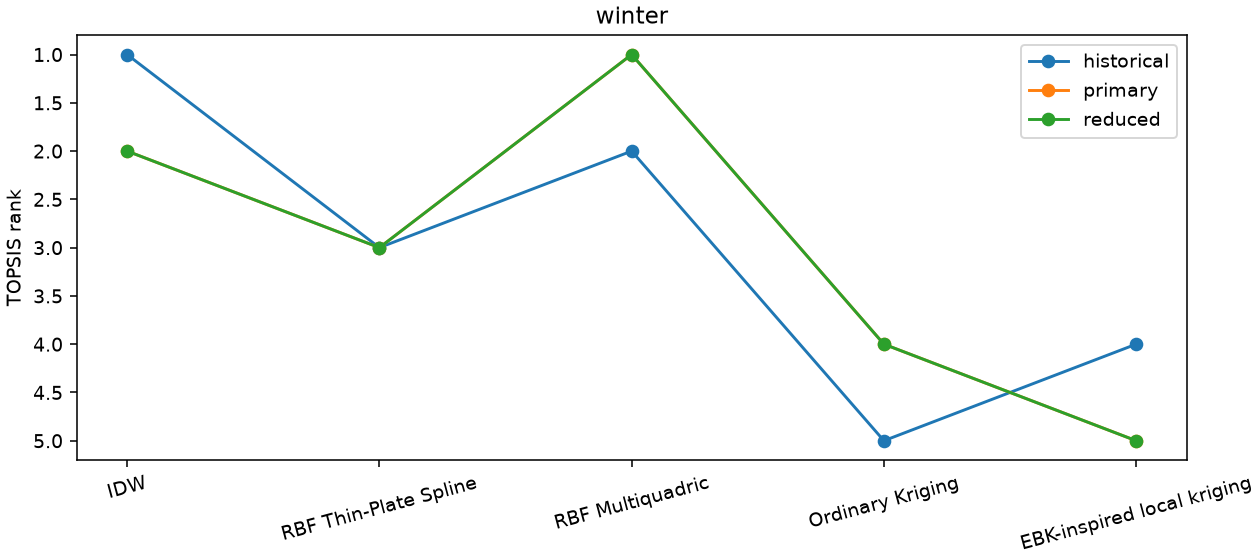
\includegraphics[width=.94\linewidth]{rankings/winter.png}\caption{Winter TOPSIS ranks under historical, primary and reduced criteria.}\end{figure}
\section{Discussion and limitations}
The study has a small spatial sample, coarse reanalysis reference and no independent ground-station validation. Spatial dependence and LOOCV provide a less demanding reconstruction problem than spatial block holdout or geographic extrapolation. Multiyear climatologies do not assess individual-year forecasts, trends or daily extremes. Equal monthly weights and pooled DJF differ from day-weighted or complete-winter means. The output grid increases map sampling only. Only IDW uses elevation and its constant lapse rate is not estimated; the different physical definitions of SRTM orthometric and ERA5 geopotential heights are not reconciled by a calibrated conversion. Fixed isotropic covariance assumptions, untuned parameters, raw RBF boundary behavior and distance-unit sensitivity limit generality. Normal-score clipping, back-transform bias, the pseudo-target and short dependent chains limit the fifth method. No uncertainty calibration or commercial EBK equivalence is claimed. TOPSIS criterion dependence and redundancy limit interpretation, and there is no independent post-selection performance estimate.

\section{Conclusion}
For the supplied ERA5-derived climatologies, multiquadric RBF performs well under the specified fixed configurations and IDW is competitive in winter. The conclusions apply only to reconstruction of this 23-location reanalysis subset. Alternative variograms, covariates, samples and validation protocols may change the ordering. No new interpolation method or TOPSIS contribution is claimed.

\paragraph{Reproducibility.} The repository supplies the configuration, explicit random streams, input hashes, held-out predictions, metric tables, ranking tables and numerical tests. Evaluation of all five methods requires only ERA5 and the authorized local geographical mask. Full IDW mapping uses the documented replacement SRTM elevations, obtainable through the public download and preprocessing scripts.

\section*{Acknowledgments}
The author acknowledges supervision by Mahboubeh Molavi-Arabshahi at Iran University of Science and Technology. Contains modified Copernicus Climate Change Service information (ERA5, 2015--2024). Neither the European Commission nor ECMWF is responsible for use of the information. GADM supports local masking; NASA/NGA SRTM data were accessed through OpenTopography, whose contribution and dataset citation are acknowledged in~\cite{opentopo}. The software's MIT license does not override third-party data permissions.
\begingroup\small
\setlength{\parskip}{2pt}
\begin{thebibliography}{99}\setlength{\itemsep}{2pt}
\bibitem{yang} R. Yang and B. Xing. A comparison of the performance of different interpolation methods in replicating rainfall magnitudes under different climatic conditions in Chongqing Province (China). \textit{Atmosphere}, 12(10), 1318, 2021. \url{https://doi.org/10.3390/atmos12101318}.
\bibitem{nash} J. E. Nash and J. V. Sutcliffe. River flow forecasting through conceptual models part I --- A discussion of principles. \textit{Journal of Hydrology}, 10(3), 282--290, 1970. \url{https://doi.org/10.1016/0022-1694(70)90255-6}.
\bibitem{era5} Copernicus Climate Change Service / ECMWF. ERA5 monthly averaged data on single levels from 1940 to present. \url{https://doi.org/10.24381/cds.f17050d7}.
\bibitem{rbf} SciPy. \texttt{Rbf} API reference. \url{https://docs.scipy.org/doc/scipy/reference/generated/scipy.interpolate.Rbf.html}.
\bibitem{ebk} Esri. What is empirical Bayesian kriging? ArcGIS Pro documentation. \url{https://pro.arcgis.com/en/pro-app/3.3/help/analysis/geostatistical-analyst/what-is-empirical-bayesian-kriging-.htm}.
\bibitem{spearman} SciPy. \texttt{spearmanr} API reference. \url{https://docs.scipy.org/doc/scipy/reference/generated/scipy.stats.spearmanr.html}.
\bibitem{gadm} GADM. License. \url{https://gadm.org/license.html}.
\bibitem{srtm} U.S. Geological Survey, Earth Resources Observation and Science (EROS) Center. SRTM 1 Arc-Second Global. \url{https://doi.org/10.5066/F7PR7TFT}.
\bibitem{opentopo} NASA Shuttle Radar Topography Mission (SRTM) (2013). Shuttle Radar Topography Mission (SRTM) Global, GL1 version 3. Distributed by OpenTopography. \url{https://doi.org/10.5069/G9445JDF}. Accessed 27 November 2026.
\bibitem{ecmwf} ECMWF. ERA5 data documentation: geopotential height and spatial reference systems. \url{https://confluence.ecmwf.int/display/CKB/ERA5%3A+data+documentation}.
\end{thebibliography}
\endgroup
\clearpage
\appendix
\section{Seasonal reconstruction maps and metrics}
\small
\setlength{\intextsep}{5pt}
\captionsetup{skip=3pt}
Maps and tables show all five configurations. IDW maps use the documented replacement SRTM elevations; each period shares a common colour scale across methods.
\subsection{Spring}
\begin{figure}[H]\centering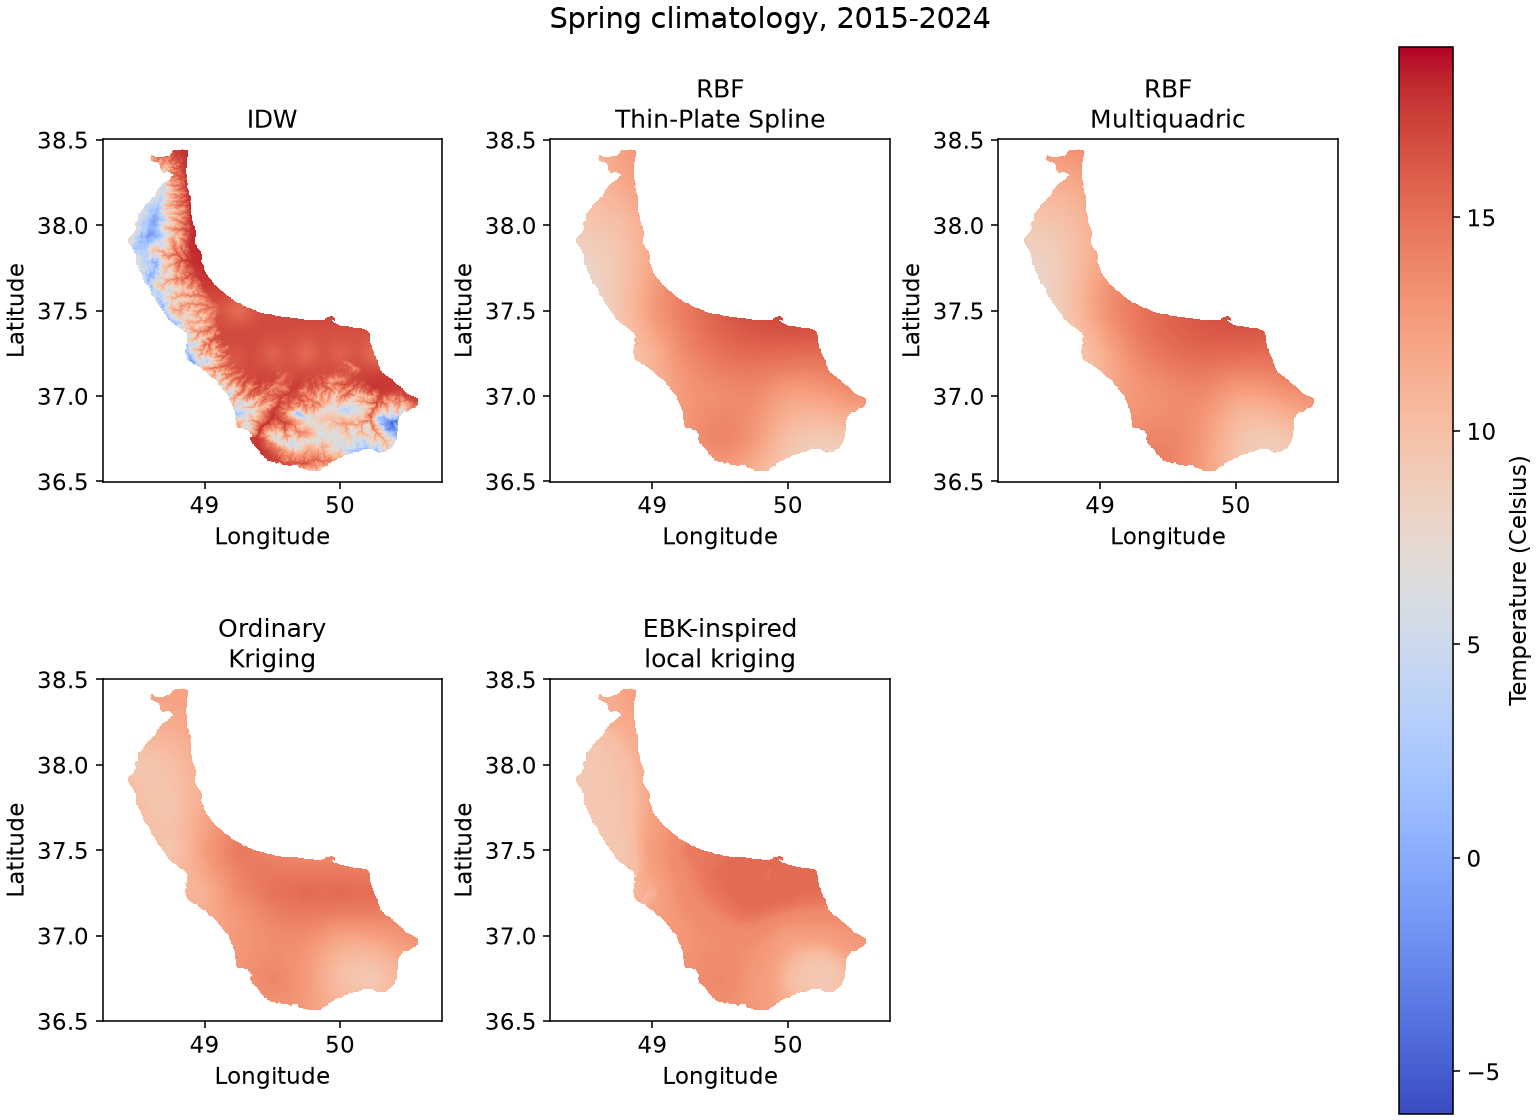
\includegraphics[width=.94\linewidth]{temperature_maps/spring.png}\caption{Spring temperature reconstruction (five configurations; replacement SRTM for IDW; \degC).}\end{figure}
\begin{table}[H]\centering\caption{Spring LOOCV metrics (MAE and RMSE in \degC).}\begin{tabular}{lrrrr}\toprule Method & MAE & RMSE & NSE & Spearman\\\midrule
IDW & 1.1677 & 1.3593 & 0.5503 & 0.9328\\
RBF thin-plate & 0.5817 & 0.7910 & 0.8477 & 0.9368\\
RBF multiquadric & 0.3743 & 0.4498 & 0.9507 & 0.9605\\
Ordinary kriging & 0.8838 & 1.0721 & 0.7202 & 0.9091\\
EBK-inspired local kriging & 0.7576 & 1.0169 & 0.7483 & 0.8449\\
\bottomrule\end{tabular}\end{table}
\clearpage\subsection{Summer}
\begin{figure}[H]\centering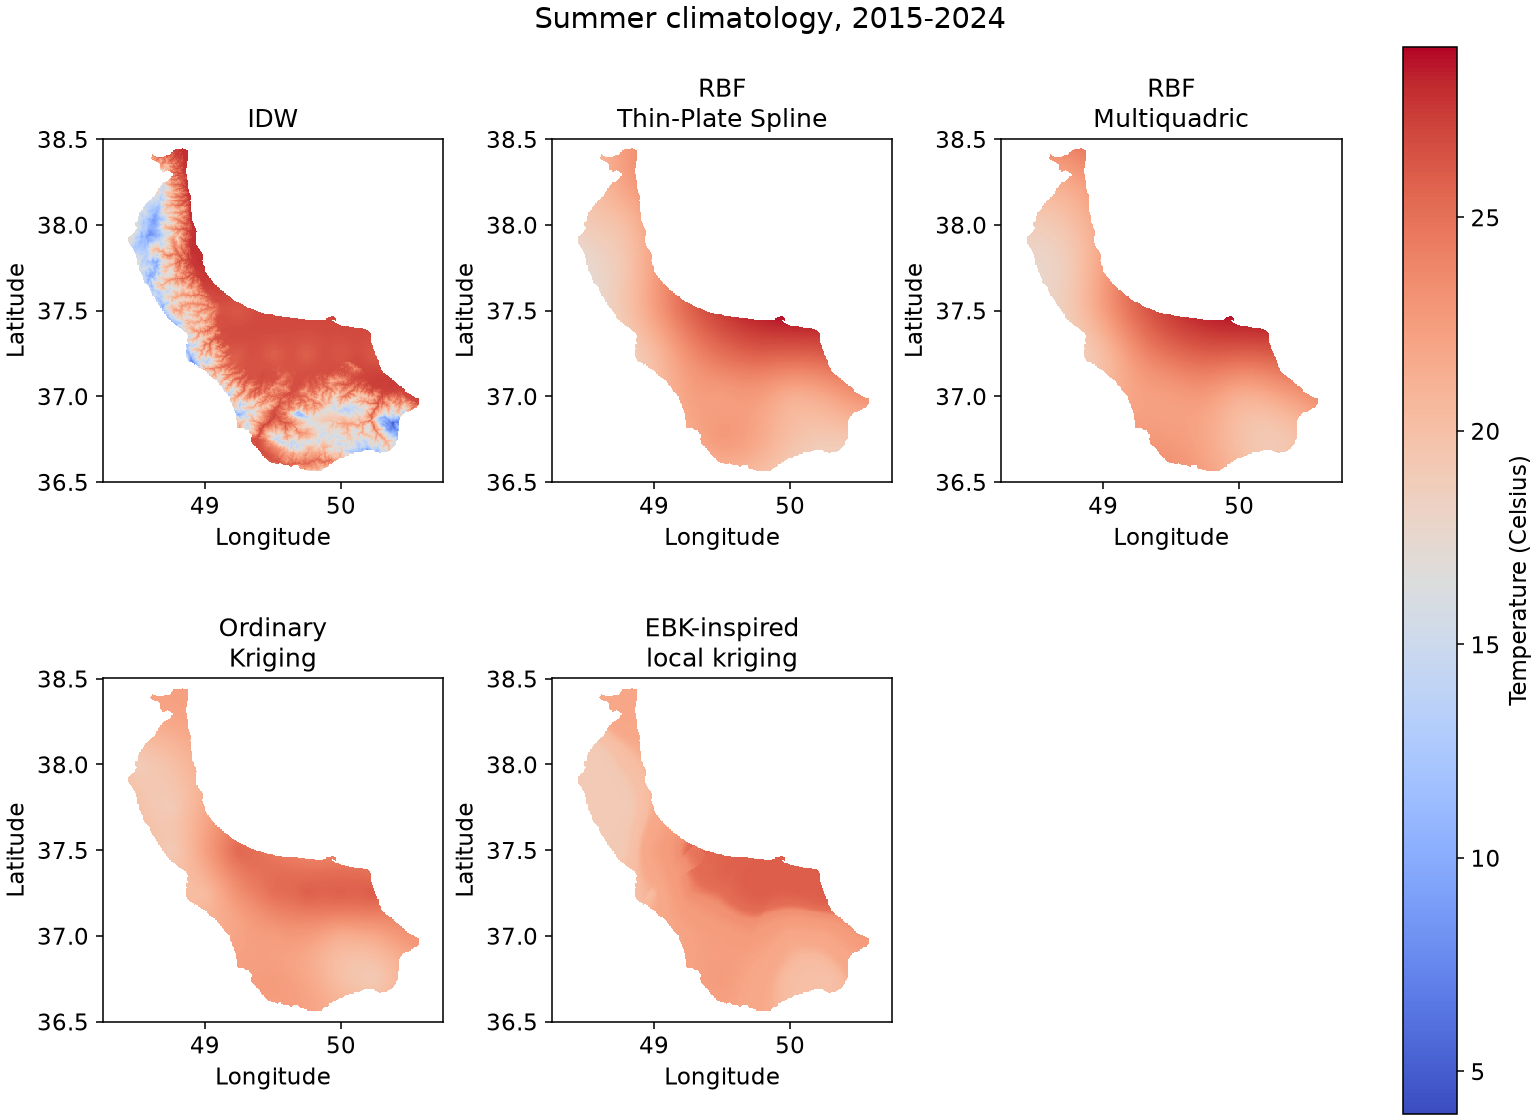
\includegraphics[width=.94\linewidth]{temperature_maps/summer.png}\caption{Summer temperature reconstruction (five configurations; replacement SRTM for IDW; \degC).}\end{figure}
\begin{table}[H]\centering\caption{Summer LOOCV metrics (MAE and RMSE in \degC).}\begin{tabular}{lrrrr}\toprule Method & MAE & RMSE & NSE & Spearman\\\midrule
IDW & 0.9395 & 1.1200 & 0.7514 & 0.9654\\
RBF thin-plate & 0.6335 & 0.8938 & 0.8417 & 0.9042\\
RBF multiquadric & 0.3841 & 0.4934 & 0.9517 & 0.9496\\
Ordinary kriging & 0.9881 & 1.2447 & 0.6929 & 0.8587\\
EBK-inspired local kriging & 1.0112 & 1.2705 & 0.6801 & 0.8251\\
\bottomrule\end{tabular}\end{table}
\clearpage\subsection{Fall}
\begin{figure}[H]\centering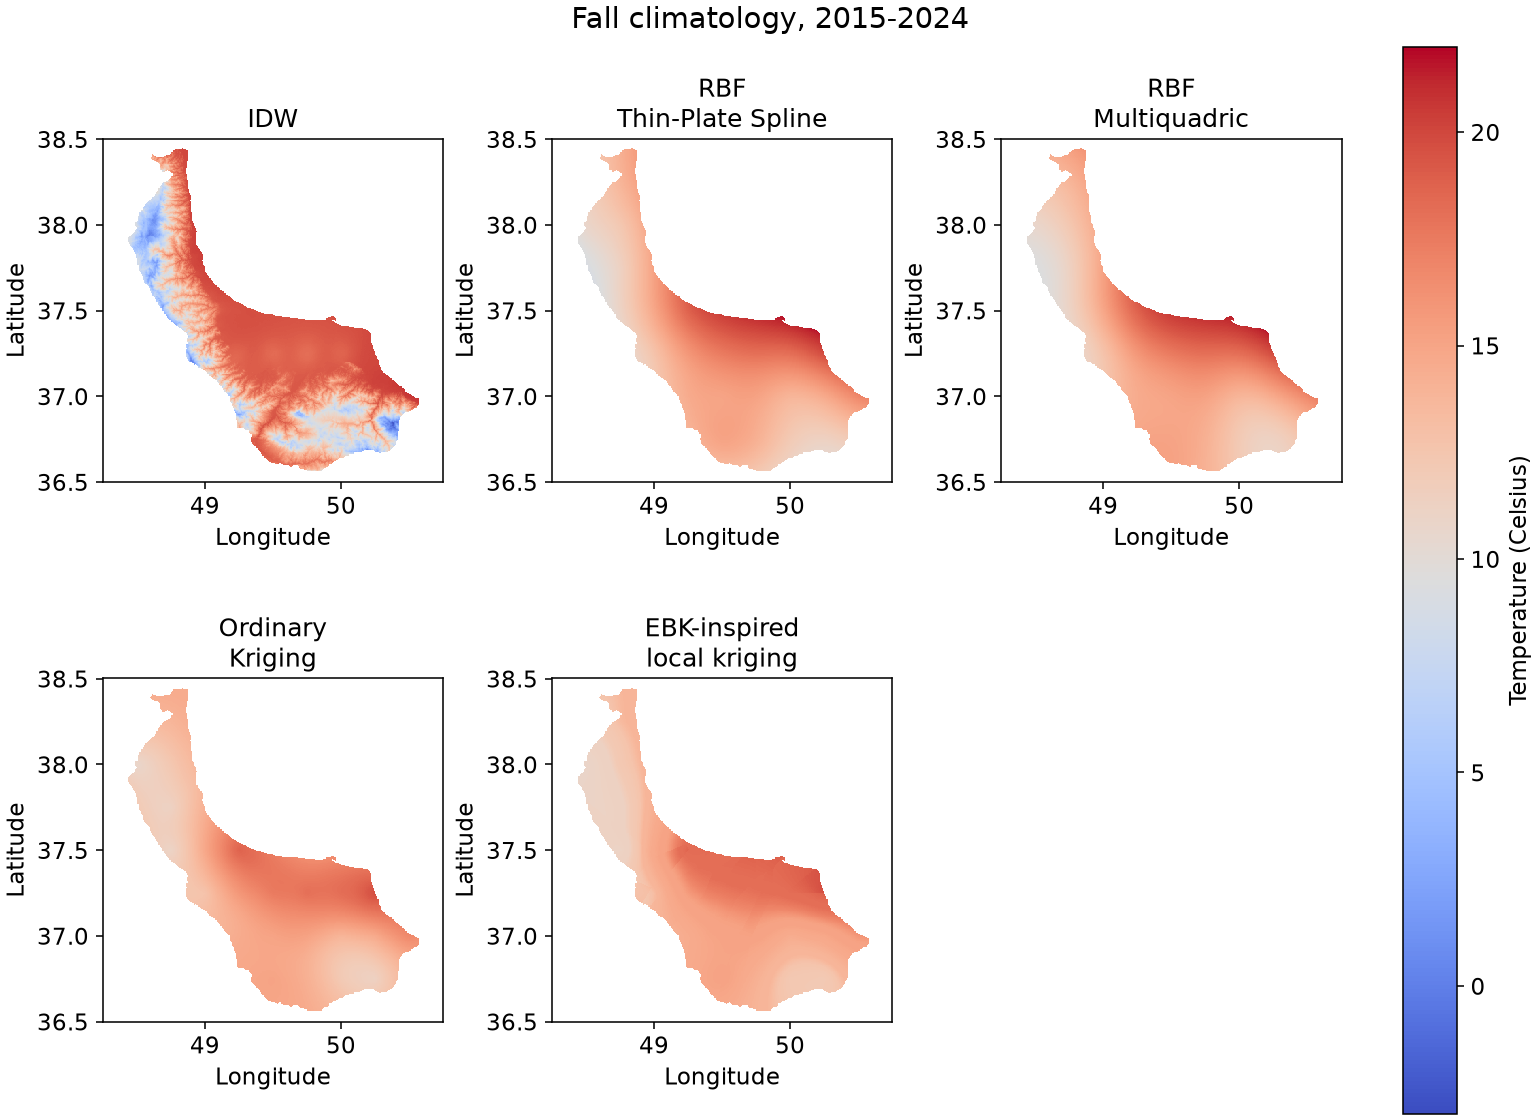
\includegraphics[width=.94\linewidth]{temperature_maps/fall.png}\caption{Fall temperature reconstruction (five configurations; replacement SRTM for IDW; \degC).}\end{figure}
\begin{table}[H]\centering\caption{Fall LOOCV metrics (MAE and RMSE in \degC).}\begin{tabular}{lrrrr}\toprule Method & MAE & RMSE & NSE & Spearman\\\midrule
IDW & 0.7291 & 0.9186 & 0.8702 & 0.9674\\
RBF thin-plate & 0.6489 & 0.8944 & 0.8770 & 0.9644\\
RBF multiquadric & 0.3946 & 0.4869 & 0.9635 & 0.9753\\
Ordinary kriging & 1.1312 & 1.5363 & 0.6371 & 0.9002\\
EBK-inspired local kriging & 1.2207 & 1.5527 & 0.6293 & 0.8261\\
\bottomrule\end{tabular}\end{table}
\clearpage\subsection{Winter}
\begin{figure}[H]\centering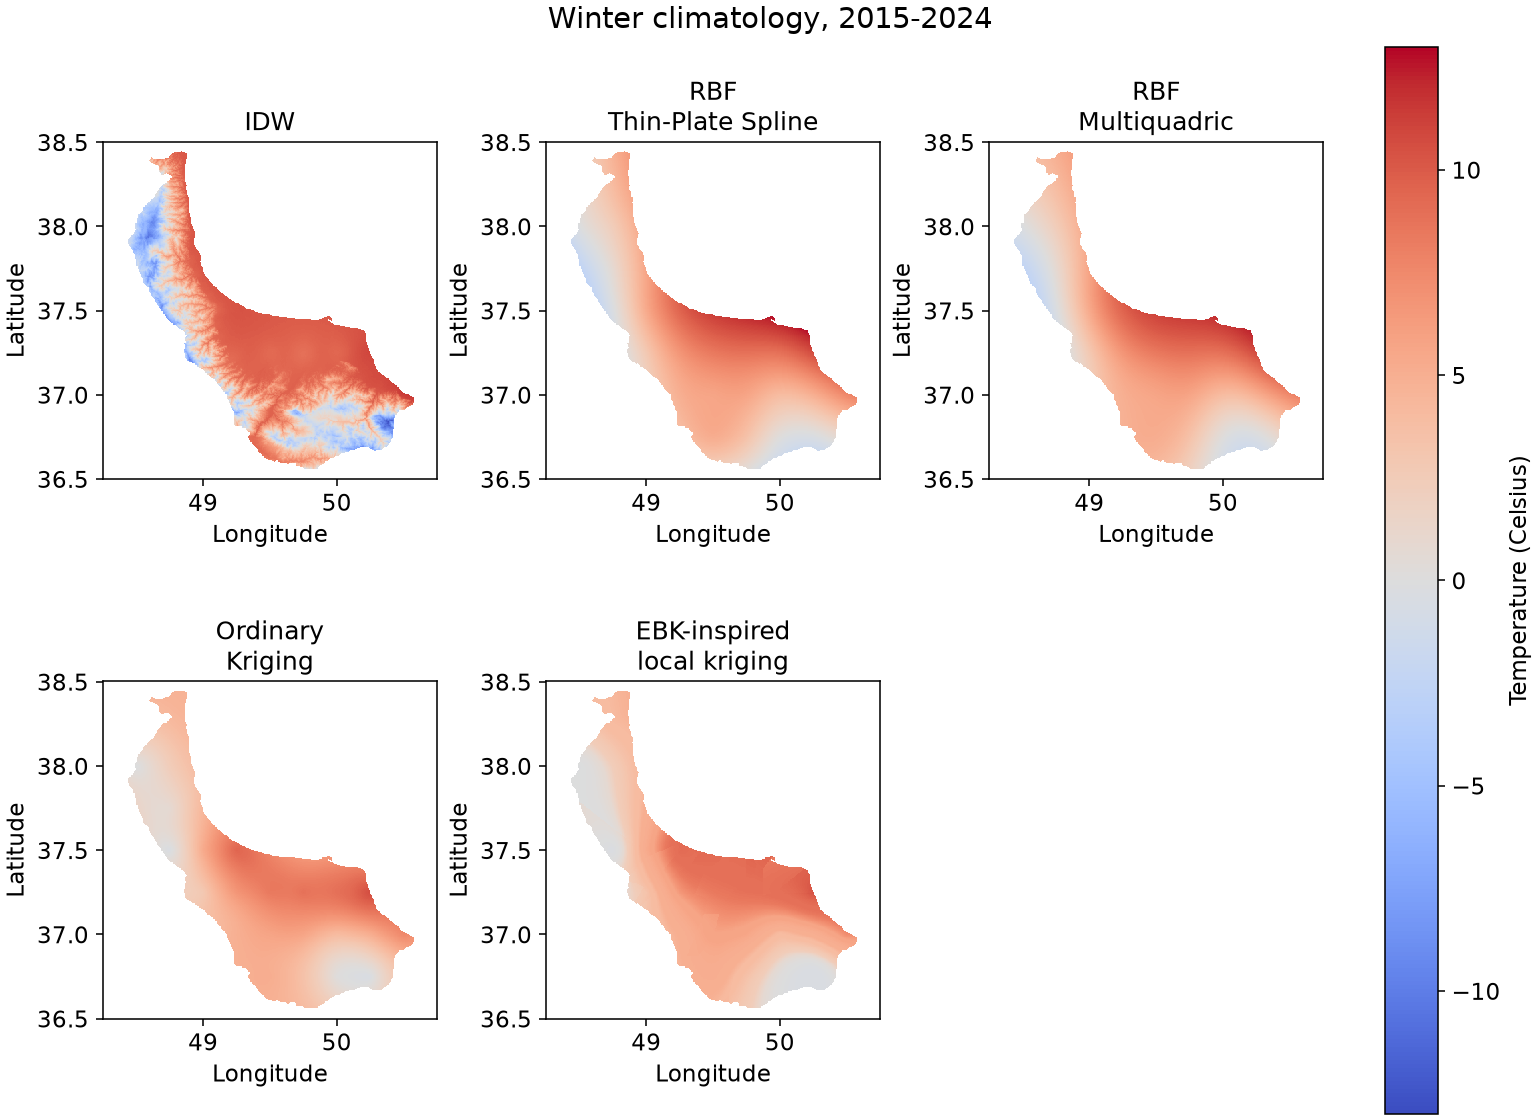
\includegraphics[width=.94\linewidth]{temperature_maps/winter.png}\caption{Winter temperature reconstruction (five configurations; replacement SRTM for IDW; \degC).}\end{figure}
\begin{table}[H]\centering\caption{Winter LOOCV metrics (MAE and RMSE in \degC).}\begin{tabular}{lrrrr}\toprule Method & MAE & RMSE & NSE & Spearman\\\midrule
IDW & 0.4095 & 0.5072 & 0.9759 & 0.9852\\
RBF thin-plate & 0.7200 & 0.9689 & 0.9119 & 0.9694\\
RBF multiquadric & 0.4099 & 0.4969 & 0.9768 & 0.9891\\
Ordinary kriging & 1.4474 & 1.9306 & 0.6502 & 0.8953\\
EBK-inspired local kriging & 1.3701 & 1.8071 & 0.6935 & 0.8607\\
\bottomrule\end{tabular}\end{table}
\end{document}
